\subsection{Exponentially decaying tails}
\subsubsection{Construction}

The first variation of the $N$-branching random walk that we consider is very similar to the one studied in \cite{exp_tails} by Bérard and Gouéré. However, we treat a slightly more general case where the number of offspring of each particle is random as opposed to being fixed at two. In this version of the $N$-branching random walk each particle dies and gives birth to a random number of offspring whose number is distributed like $q$. Given the position of the parent, say $x$, each child's position follows the law $p(\,\cdot - x)$ independently of the number and position of the other children. 

\begin{construction} Let $X = (X_n)_{n \geq 0} = (\sum_{i = 1}^N \delta_{X_n(i)})_{n \geq 0}$ denote the $\frak{M}_N$-valued discrete time Markov process defined by the branching-selection procedure detailed above. Note that we suppress the dependence on $N$ in our notation for simplicity. We can construct $X$ easily: Let $\cal{E}_N \defeq (\epsilon_{l, i, j})_{l \geq 0,\,i \in [N],\,j \geq 1}$ and $\cal{M}_N \defeq (\tau_{l, i})_{l \geq 0, i \in [N]}$ be i.i.d. collections of random variables distributed like $p$ and $q$ respectively, with the collections also independent from each other. Now, given the process up to time $n \geq 0$, we construct $X_{n+1}$ as follows: define $Y_{n+1} \defeq \sum_{i = 1}^N \sum_{j=1}^{\tau_{n, i}} \delta_{X_n(i) + \epsilon_{n, i, j}}$ and take $X_{n+1}$ to given by the $N$ rightmost particles of $Y_{n+1}$. 
\end{construction}

Let $\nu \in \frak{M}$ be a random, finite counting measure with the same distribution as the offspring of a single particle at the origin in our branching-selection mechanism (the fact that $\nu \in \frak{M}$ follows from Assumption \ref{ass:offspring}). In other words, the number of atoms of $\nu$ has distribution $q$ and each atom is placed independently at position drawn from $p$. Let us now define the logarithmic moment generation function of $\nu$: 
\begin{equation*}
\psi(t) \defeq \log \E\int_\R e^{tx} d\nu (x).  
\end{equation*}
Note that in their analysis Bérard and Gouéré define a slightly different function $\Lambda(t) = \psi(t) - \log 2$, however the branching random walk literature usually uses our definition. We impose the following assumptions to gain access to the results of \cite{gantert2008asymptotics}:
\begin{assumption}\label{ass:exponential_tails}
$\psi$ is finite in some neighbourhood of $0$. 
\end{assumption}
\begin{assumption}\label{ass:weird}
There exists $t^* > 0$ in the interior of the domain of $\psi$ such that $t^*\psi'(t^*) = \psi(t^*)$. 
\end{assumption}

Assumption \ref{ass:exponential_tails} is in fact equivalent to the requirement that $p$ have exponentially decaying tails, furthermore it implies that $p$ has finite moments of all orders. The third assumption concerns the distribution $q$: 
\begin{assumption}\label{ass:offspring}
$q$ satistfies $q(0) = 0$ and $1 < \sum_{i = 1}^\infty i^2 q(i) < \infty$. 
\end{assumption}

The results that follow in this section are conditional upon Assumptions \ref{ass:exponential_tails}, \ref{ass:weird} and \ref{ass:offspring} being satisfied. We now record a technical lemma that will help us later. \\
\begin{lemma}\label{lem:ExpTailsMax}
Let $\tau \in L^1$ be an $\N$-valued random variable and let $(\epsilon_n)_{n \geq 1}$ be an i.i.d. sequence of random variables with exponentially decaying tails, independent of $\tau$. Then $M \defeq \max_{1 \leq n \leq \tau} \epsilon_n$ has exponentially decaying tails. 
\end{lemma}

\begin{proof}
Let $C, \gamma, t_0 > 0$ be such that $\Pr{|\epsilon_1| \leq t} \geq 1 - C e^{- \gamma t}$ for all $t > t_0$. Then for $t > t_0$ large enough, Bernoulli's inequality gives 
\begin{align*}
\Pr{M > t} &\leq 1 - \Ex{\Pr{|\epsilon_1| \leq t}^\tau} \leq 1 - \Ex{(1 - C e^{-\gamma t})^\tau} \\
		   &\leq 1 - \Ex{1 - C e^{- \gamma t} \tau} = \underbrace{C\, \Ex{\tau}}_{< \infty} e^{- \gamma t}. 
\intertext{Similarly, looking at the lower tail we get}
\Pr{M < -t} &\leq 1 - \Ex{\Pr{|\epsilon_1| \leq t}^\tau} \leq C\, \Ex{\tau} e^{- \gamma t}. 
\end{align*}
\end{proof}

% \begin{wrapfigure}{R}{0.5\textwidth}
% \centering
% 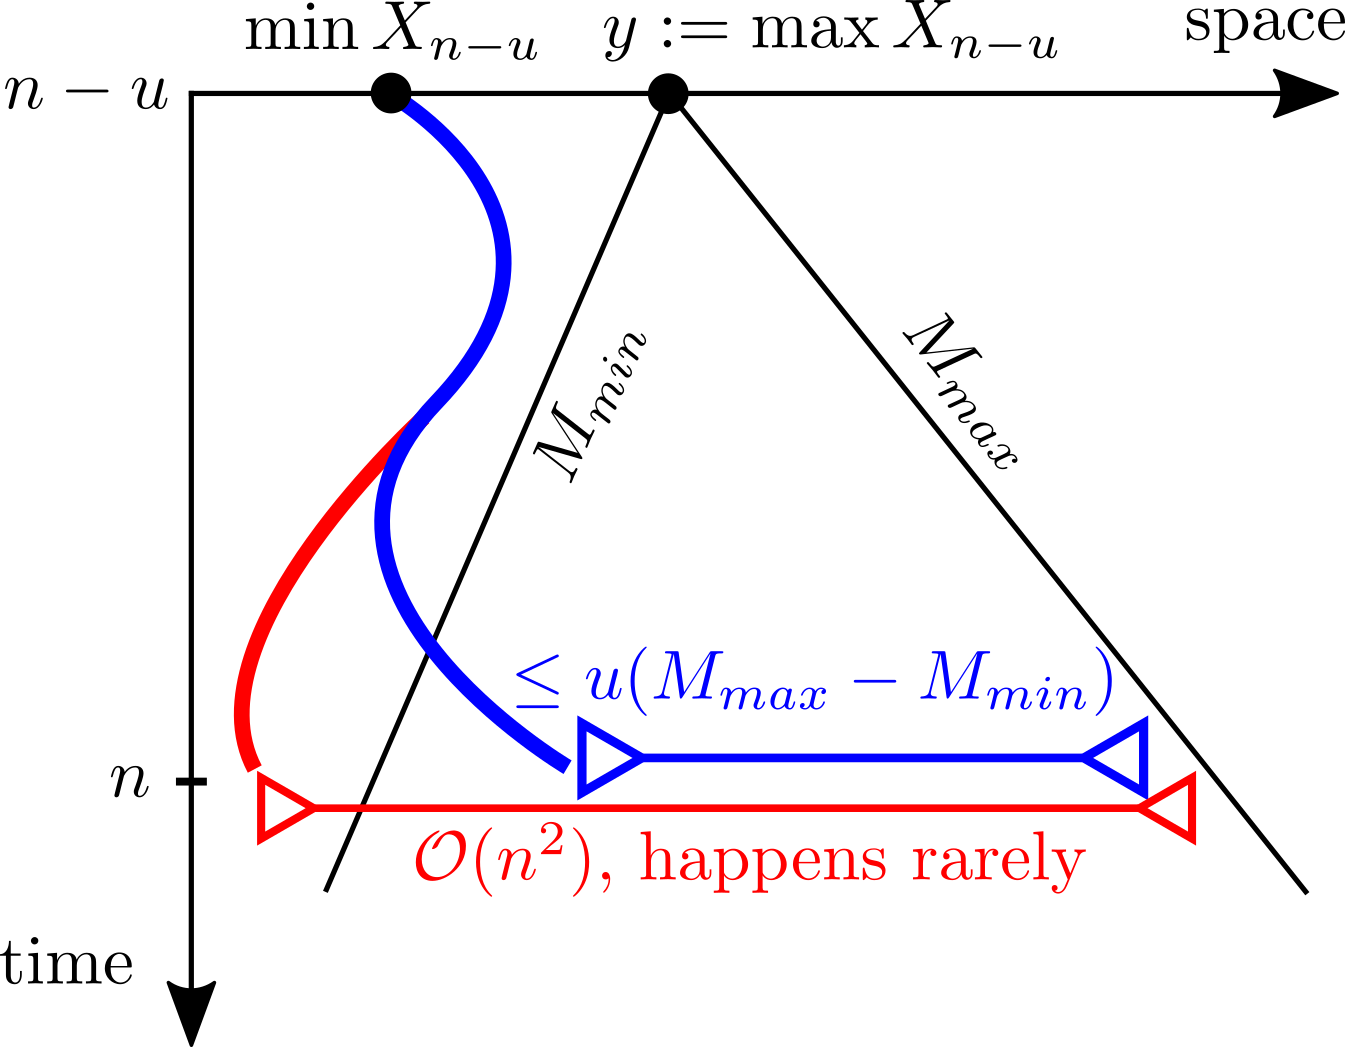
\includegraphics[width=0.45\textwidth]{graphics/g2.png}
% % \caption{\label{fig:frog1}This is a figure caption.}
% \end{wrapfigure}

\subsubsection{Properties of the model}
Denote by $\max X_n$ and $\min X_n$ the position of the right- and leftmost particle of $X_n$ respectively. It is worth noting that $\min X_n$ and $\max X_n$ are integrable and hence finite by Assumptions \ref{ass:exponential_tails} and \ref{ass:offspring} when started from any fixed $X_0 \in \frak{M}_N$. Indeed, by independence we have 
\begin{equation}\label{eqn:ExpTailsMaxIntegrable}
\E|\max X_n| \leq \E\left\vert\max X_0 + \sum\limits_{l=0}^{n-1} \sum\limits_{i=1}^N \sum\limits_{j=1}^{\tau_{l,i}} \epsilon_{l,i,j} \right\vert \leq |\max X_0| + N n \Ex{\tau_{0,1}} \E|\epsilon_{0, 1, 1}|. 
\end{equation}
Denote by $d(X_n) \defeq \max X_n - \min X_n$ the diameter of $X_n$. We have the following result, analogous to Corollary 1 of \cite{exp_tails}: 

\begin{proposition}\label{prop:diameter}
For any $N \geq 1$ and initial population $X_0 \in \frak{M}_N$, we have 
\begin{equation*}
\frac{d(X_n)}{n} \xrightarrow[n \to \infty]{a.s.,\, L^1} 0. 
\end{equation*}
\end{proposition}

\begin{proof}
Let $u \in \N_+$ and for $n \geq u$ consider the process $X$ in the timeframe $\bbracket{n - u, n}$. Define $\cal{E} \defeq \{ \epsilon_{l, i, j} \mid\, l \in \bbracket{n - u,n - 1},\, i \in [N],\, j \in [\tau_{l,i}] \}$ and let $M \defeq \max \cal{E}$, $m \defeq \min \cal{E}$ noting that both have exponentially decaying tails by Lemma \ref{lem:ExpTailsMax}. Write $y \defeq \max X_{n - u}$ for the rightmost particle's position at time $n-u$. Suppose that for each $k \in [u]$ we have $\min X_{n - u + k} < y + k m$. As all steps during branching are $ \geq m$, this implies in particular that the descendants of the particle `$y$' survive all selection steps until time $n$. Therefore, on the event $A_u \defeq \{ \text{number of descendants of } y \text{ at time } n \text{ is } > N\}$ almost surely $\min X_{n - u + k} \geq y + k_0 m$ for some $k_0$. By the definition of $m$ this must also hold for all $k \in \bbracket{k_0, u}$, in particular for $k = u$. Noting that $\max X_n \leq y + u M$, it follows that 
\begin{equation}\label{eqn:ExpTailDiamUpperBound}
d(X_n)\Ind_{A_u} \leq u (M - m), 
\end{equation}
with probability one. A simple argument shows that $\Ind_{A_u} \to 1$ almost surely as $u \uparrow \infty$: take any path of length $u$ started from `$y$'. On $A_u^c$, along any such path the number of times that the corresponding particle has more than one child is less than $N$. 
\begin{equation}
\Pr{A^c_u} \leq \sum\limits_{k = 0}^{N - 1} {u \choose k} q(1)^{u - k} (1 - q(1))^k \leq N u^{N-1} q(1)^{u - (N - 1)} \to 0 
\end{equation}
as $u \uparrow \infty$ since $q(1) < 1$. Fix $\epsilon > 0$ and take $u$ large enough so that $\Pr{A_u^c} < \epsilon^2$. Consider the decomposition
\begin{equation}\label{eqn:ExpTailsDiamDecomp}
\frac{d(X_n)}{n} = \frac{d(X_n)}{n} \Ind_{A_u} + \frac{d(X_n)}{n} \Ind_{A_u^c}. 
\end{equation}
Taking expectations and then taking $n$ to infinity, the first term vanishes by (\ref{eqn:ExpTailDiamUpperBound}). The second term is upper bounded by $(\Pr{A_u^c} \Ex{d(X_n)^2 / n^2})^{1/2}$ using Hölder's inequality. A rough bound on $d(X_n)$ suffices now: at each branching step $l \geq 0$ take the maximum and the minimum of the $\sum_{j=1}^N \tau_{l, j}$ random walk steps. The diameter certainly grows by no more than the difference between these two at each step. By Lemma \ref{lem:ExpTailsMax} this yields $\Ex{d(X_n)^2} = \cal{O}(n^2)$ which implies that the second term in \ref{eqn:ExpTailsDiamDecomp} is $\cal{O}(\epsilon)$. Taking $\epsilon$ to zero concludes the proof of $L^1$ convergence. Almost sure convergence is a consequence of the proof of the next Proposition. 
\end{proof}

\begin{proposition}[{{\cite[Proposition 2]{exp_tails}}}]\label{prop:ExpTailsSpeedExistence}
There exists $v_N = v_N(p) \in \R$ such that for any initial population $X_0 \in \frak{M}_N$ the following holds almost surely and in $L^1$:
\begin{equation}
\lim\limits_{n \to \infty} \frac{\min X_n}{n} = \lim\limits_{n \to \infty} \frac{\max X_n}{n} = v_N. 
\end{equation}
\end{proposition}

\begin{proof}
First we treat the case $X_0 = N \delta_0$. Recall the definition of $\cal{E}_N$ and $\cal{M}_N$ from the construction of $X$. For each $l \geq 0$ we define the process $(X^l_n)_{n \geq 0}$ by shifting the origin of time by $l$. More precisely, given the process up to time $n \geq 0$, define $X^l_{n+1}$ to be given by the $N$ rightmost particles of $\sum_{i = 1}^N \sum_{j=1}^{\tau_{n + l,i}} \delta_{X^l_n(i) + \epsilon_{n + l, i, j}}$. It is clear that each $(X^l_n)_{n \geq 0}$ is distributed as the $N$-branching random walk with offspring law $p$. Start $(X^l_n)_{n \geq 0}$ from $N \delta_0$ for each $l \geq 0$ so that $(X^0_n)_{n \geq 0} = (X_n)_{n \geq 0}$ almost surely. From Lemma \ref{lem:monotonicity} it follows easily that 
\begin{equation}\label{eqn:subadd}
\max X^0_{n + m} \leq \max X^0_n + \max X^n_m \qquad \forall\, n,m \geq 0. 
\end{equation}
For notational simplicity define $Y_{i,j} = \max X^i_{j - i}$ for $0 \leq i \leq j$. Then (\ref{eqn:subadd}) reads $Y_{0, j} \leq Y_{0,i} + Y_{i,j}$ for all $0 \leq i \leq j$, which is familiar territory for Kingman's Subadditive Ergodic Theorem. We postpone showing that the conditions of the theorem hold to Lemma \ref{lem:ExpTailsKingmanHolds}. Applying the theorem yields $\lim_{n \to \infty} n^{-1} \max X_n = \lim_{n \to \infty} \Ex{n^{-1} \max X_n} = \inf_n \Ex{n^{-1} \max X_n} = v_N \in \R$ where the first limit is almost sure. Noting that the process $(-X_n)_{n \geq 0}$ satisfies all the same assumptions as $X$, we can deduce from the identity $\min X_n = - \max (-X_n)$ that $\lim_{n \to \infty} n^{-1} \min X_n = \lim_{n \to \infty} \Ex{n^{-1} \min X_n} = \inf_n \Ex{n^{-1} \min X_n} = \tilde{v}_N \in \R$ exists too, where the first limit is almost sure. From the proof of Proposition \ref{prop:diameter} we immediately get $\tilde{v}_N = v_N$ by uniqueness of $L^1$ limits, which gives $\lim_{n\to\infty} n^{-1}d(X_n) = v_N - \tilde{v}_N = 0$ almost surely as claimed. The proof is complete in the case $X_0 = N \delta_0$. By translation invariance of the dynamics of the system the result also follows for initial conditions of the form $N \delta_{x_0}$ for any $x_0 \in \R$. Finally, for arbitrary $X_0 \in \frak{M}_N$ note that the result is a consequence of Lemma \ref{lem:monotonicity} and a sandwiching argument between the initial configurations $N \delta_{\min X_0}$ and $N \delta_{\max X_0}$. 
\end{proof}

\begin{wrapfigure}{R}{0.5\textwidth}
\centering
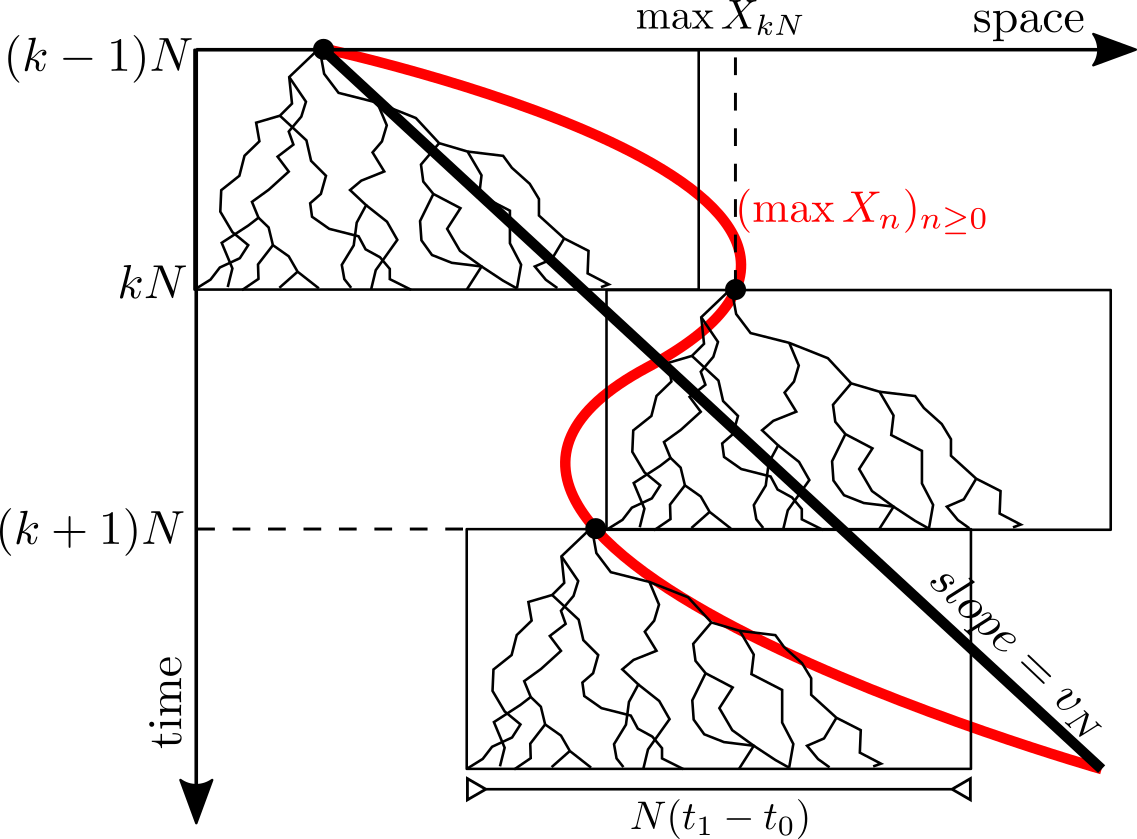
\includegraphics[width=0.45\textwidth]{graphics/g1.png}
% \caption{\label{fig:frog1}This is a figure caption.}
\end{wrapfigure}

If we look at the previous proof, we see that the existence of $v_N$ and $\tilde{v}_N$ (the almost sure and $L^1$ limits of the left- and rightmost particles) when started from $X_0 = N \delta_0$ was shown without relying on Proposition \ref{prop:diameter}. We can in fact deduce Proposition \ref{prop:diameter} by an argument inspired by one of Prof. Berestycki's suggestions:


\begin{proof}[Alternative proof of Proposition \ref{prop:diameter}]
Let $Y = (Y_n)_{n \geq 0}$ be a branching random walk (without selection) with offspring distribution $q$ and step distribution $p$. Start $Y$ from $\delta_{0}$ noting that initially there is only one particle. It is easy to see that the probability $\rho_1$ that the number of particles in $Y_n$ has reached $N$ by time $N$ is strictly positive. Similar to the proof of Proposition \ref{prop:diameter}, define $\cal{E} \defeq \{ \epsilon_j \mid\, 1 \leq i \leq \sum^{N^2}_{i=1} \tau_i,\, (\epsilon_j)_{j \geq 0} \stackrel{\mathclap{iid}}{\sim} p \perp \tau_i \stackrel{\mathclap{iid}}{\sim} q \}$ and $M \defeq \min\cal{E}, m \defeq \max\cal{E}$, where we should think of $\cal{E}$ as the set of possible random walk steps that $Y$ can take up to time $N$. By Lemma \ref{lem:ExpTailsMax} we can choose $t_0 < t_1$ such that $\rho_2 \defeq \Pr{t_0 \leq m \leq M \leq t_1} > 0$. We can now write

\begin{multline}\label{eqn:ETBC}
\Pr{\{Y_N \text{ has $N$ particles}\} \cap \{ N t_1 \geq \max Y_N \geq \min Y_N \geq N t_0\}} = \\
\qquad = \Pr{Y_N \text{ has $N$ particles}} \PrCond{N t_1 \geq \max Y_N \geq \min Y_N \geq N t_0}{Y_N \text{ has $N$ particles}} \\
\geq \rho_1 \rho_2 > 0. 
\end{multline}
Suppose that we couple $X$ with $((Y^{(k)}_n)_{0 \leq n \leq N})_{k \geq 0}$ which are independent copies of $Y$  placed at the space-time points $(\max X_{kN}, kN)_{k \geq 0}$. By the second Borel-Cantelli lemma and (\ref{eqn:ETBC}) it follows that almost surely infinitely many of the $(Y^{(k)}_n)_{0 \leq n \leq N}$ must have $N$ particles by time $N$ and have $N t_0 \leq \min Y^{(k)}_N \leq \max Y^{(k)}_N \leq N t_1$. This in turn implies that for infinitely many $k \geq 0$ the diameter $d(X_{kN})$ is less than $N(t_1 - t_0)$, which immediately yields $\tilde{v}_N = v_N$. 
\end{proof}

\begin{proposition}[{{\cite[analogue of Proposition 3]{exp_tails}}}]\label{prop:increasing_speed}
The sequence $(v_N)_{N \geq 1}$ is non-decreasing. 
\end{proposition}
\begin{proof}
This is again a consequence of Lemma \ref{lem:monotonicity}. 
\end{proof}

\begin{remark}\label{rem:constants}
From Proposition \ref{prop:increasing_speed} we can deduce that $v_N$ increases to a possibly infinite limit $v_\infty$ as $N$ goes to infinity. Assumption \ref{ass:exponential_tails} implies that $\Lambda$ is smooth on the interior of $\cal{D}(\Lambda)$ so that both quantities $v \defeq \psi'(t^*)$ and $\chi \defeq \frac{\pi^2}{2} t^* \psi''(t^*)$ are finite. In Section \ref{sec:ExpTails_BrunDer} we will see that $v_\infty$ is in fact equal to $v$. 
\end{remark}

\begin{lemma}\label{lem:ExpTailsKingmanHolds}
The random variables $Y_{i,j}$ as defined in the proof of Proposition \ref{prop:ExpTailsSpeedExistence} satisfy the hypothesis of Kingman's Subadditive Theorem. 
\end{lemma}

\begin{proof}
For each $k \geq 1$ the sequence $\{Y_{k, 2k}, Y_{2k, 3k}, ...\} = \{\max X^k_k, \max X^{2k}_k, ... \}$ is i.i.d. so stationary and ergodic. Clearly the distribution of $(Y_{i, i + k})_{k \geq 0} = (\max X^i_k)_{k \geq 0}$ is independent of $i$. $\E Y^+_{0,1} = \E (\max X_1)^+ < \infty$ because $\max X_1 \in L^1$ by (\ref{eqn:ExpTailsMaxIntegrable}). Finally, $\E Y_{0, n} = \E \max X_n \geq n\, \E \min\{\epsilon_{0, i, j} \mid\, i \in [N],\, j \in [\tau_{0, i}]\}$ where the expectation is finite by Lemma \ref{lem:ExpTailsMax}. 
\end{proof}

\subsubsection{Killed branching random walks}
Adapting the notation used in \cite{exp_tails}, we formally define a Branching Random Walk (BRW) to be a pair $(\cal{T}, \Phi)$, where $\cal{T}$ is a Galton-Watson tree with offspring distribution $q$ and $\Phi$ is a map assigning a random variable $\Phi(u)$ to each vertex $u \in \cal{T}$, independently of the structure of $\cal{T}$. $\Phi$ must be such that  $\Phi(\text{root}) = 0$ and $\{\Phi(v) - \Phi(u) \mid\, \text{$u$ is the parent of $v$}\}$ is an i.i.d. collection with common distribution $p$. We call $\Phi(u)$ the value of the BRW at vertex $u$ and write $\cal{T}(n)$ for the set of vertices in $\cal{T}$ at depth $n$. We say a (possibly finite) sequence of vertices $u_1, u_2, ...$ is a path if $u_{i+1}$ is the parent of $u_i$ for each $i \geq 1$. \\
Suppose that we have a BRW $(\cal{T}, \Phi)$ and take $v \in \R$ and $m \geq 1$. We say that vertex $u$ is $(m, v)$-good if there exists a path $u = u_0, u_1, ..., u_m$ such that $\Phi(u_i) - \Phi(u) \geq vi$ for all $i \in \bbracket{0,m}$. This is essentially saying that there exists a path started from $u$ that stays to the right of the space-time line through $(u, \Phi(u))$ with slope $v$, for at least $m$ steps. The definition of an $(\infty, v)$-good vertex is analogous. We now state two results from \cite{gantert2008asymptotics} that we will need to prove Theorem \ref{thm:ExpTails_BrunDer}. Recall the definitions of $v$ and $\chi$ from Remark \ref{rem:constants}. 

\begin{theorem}[{{\cite[Theorem 1.2]{gantert2008asymptotics}}}]\label{thm:infty_good}
Let $\rho(\infty, \epsilon)$ denote the probability that the root of the BRW with offspring distribution $q$ and step distribution $p$ is $(\infty, v - \epsilon)-good$. Then, as $\epsilon > 0$ goes to zero, 
\begin{equation}
\rho(\infty, \epsilon) \leq \exp\left( - \left( \frac{\chi + o(1)}{\epsilon} \right)^{1/2} \right). 
\end{equation}
\end{theorem}

A similar result can be stated for the probability of observing a $(m, v - \epsilon)$-good root with $m$ finite:
\begin{theorem}[{{\cite[Consequence of proof of Theorem 1.2]{gantert2008asymptotics}}}]\label{thm:finite_good}
Let $\rho(m, \epsilon)$ denote the probability that the root of the BRW with offspring distribution $q$ and step distribution $p$ is $(m, v - \epsilon)$-good. For any $0 < \beta < \chi$, there exists $\theta > 0$ such that for all large $m$, 
\begin{equation*}
\rho(m, \epsilon) \leq \exp\left( - \left( \frac{\chi - \beta}{\epsilon} \right)^{1/2} \right), \qquad \text{with } \epsilon \defeq \theta m^{-2/3}. 
\end{equation*}
\end{theorem}

\subsubsection{Brunet-Derrida behaviour}\label{sec:ExpTails_BrunDer}

We are now ready to present and prove our main result in this section, the analogue of Bérard and Gouéré's Theorem 1:
\begin{theorem}\label{thm:ExpTails_BrunDer}
As $N$ goes to infinity, 
\begin{equation*}
v_\infty - v_N = \frac{\chi}{(\log N)^2} + o((\log N)^{-2}). 
\end{equation*}
\end{theorem}

First let us describe the coupling between the $N$-branching random walk and $N$ independent branching random walks which allows us to relate Theorems \ref{thm:infty_good} and \ref{thm:finite_good} to the $N$-branching random walk. Let $(\text{BRW}_i)_{i \in [N]} = ((\cal{T}_i, \Phi_i))_{i \in [N]}$ be a set of $N$ independent copies of the BRW with offspring distribution $q$ and step distribution $p$. Define $\bb{T}_n \defeq \bigsqcup_{i=1}^N \cal{T}_i(n)$ to be the disjoint union of vertices at depth $n$ in the $N$ BRWs, and fix an arbitrary (nonrandom) total order on $\bb{T}_n$ for each $n$. We now inductively define a sequence $(G_n)_{n \geq 0}$ of random subsets of $\bb{T}_n$, each with exactly $N$ elements. These random subsets will correspond to the particles alive in the coupled $N$-braching random walk at time $n$. Define $G_0 = \bb{T}_0$ and given $G_n$, define $H_n$ to be the vertices in $\bb{T}_{n+1}$ that descend from vertices in $G_n$. Finally, set $G_{n+1}$ to be the set of $N$ vertices in $H_n$ with the gratest value, resolving ties via the fixed total order on $\bb{T}_{n+1}$. If we now define (with some abuse of notation) $\frak{X}_n = \sum_{u,i : u \in G_n \cap \cal{T}_i} \delta_{\Phi_i(u)}$ then $(\frak{X}_n)_{n \geq 0}$ has the same distribution as $X$ started from $N \delta_0$. Going forward we will alternate between the notation of the two constructions of the $N$-branching random walk that we have given. Concretely, we will refer to $\cal{T}$, $\Phi$, $\epsilon_{n,i,j}$ and $\tau_{n,i}$ without explicitly explaining the obvious relationships between these objects. Let us now record a technical lemma that will be used in the proof of the lower bound in Theorem \ref{thm:ExpTails_BrunDer}. 

\begin{lemma}[{{\cite[Adapted by Bérard and Gouéré from Lemma 5.2]{pemantle2009search}}}]\label{lem:ExpTailsGoodSequencesTechnical}
Let $v_1 < v_2 \in \R$ and $1 \leq m \leq n \in \N$. Suppose $0 \eqdef x_0, ..., x_n$ is a sequence of real numbers such that $\max_{i \in \bbracket{0, n - 1}} (x_{i+1} - x_i) \leq K$ for some $K > 0$, and define $I \defeq \{ i \in \bbracket{0, n - m} \mid\, x_{i + j} - x_i \geq j v_1,\quad \forall j\in\bbracket{0,m}\}$. If $x_n \geq v_2 n$, then $\#I \geq \frac{v_2 - v_1}{K - v_1}\frac{n}{m} - \frac{K}{K - v_1}$. 
\end{lemma}

\begin{proof}[Proof of lower bound in Theorem \ref{thm:ExpTails_BrunDer}]
As before, we first treat the case $X_0 = N \delta_0$. Our aim is to show $v_N \defeq \lim_{n \to \infty} \Ex{n^{-1} \max X_n} \leq v_\infty - \chi / (\log N)^2 + o((\log N)^{-2})$. However, we shall show this with $v_\infty$ replaced by $v$, which combined with the upper bound also proves that $v_\infty = v$. Set $\beta \in (0, \chi)$ and let $\theta > 0$ be as in Theorem \ref{thm:finite_good}. Let $\lambda > 0$, and define 
\begin{equation}
m \defeq \ceil*{\theta^{3/2}\left( \frac{(1 + \lambda) \log N}{(\chi - \beta)^{1/2}}\right)^3},
\end{equation}
and $\epsilon \defeq \theta\, m^{-2/3}$. The scale of $m$ is carefully chosen so that by Theorem \ref{thm:finite_good}, 
\begin{equation}
\rho(m, \epsilon) \leq N^{-(1 + \lambda)} \qquad\text{for all large } N. 
\end{equation}
Take $\gamma \in (0, 1)$ and define $v_1 = v - \epsilon$ and $v_2 = v - (1 - \gamma) \epsilon$ noting that $v_1 < v_2 < v$. Finally, let $n = \ceil{N^\xi}$ for some $0 < \xi < \lambda$ and consider the following inequality with $\delta > 0$:
\begin{align}
\Ex{n^{-1} \max X_n} &= \Ex{n^{-1} \max X_n \left[ \Ind_{\{ \max X_n < n v_2\}} + \Ind_{\{ n v_2 \leq \max X_n < n (v + \delta)n \}} + \Ind_{\{ (v + \delta)n \leq \max X_n \}} \right]}\nonumber \\
					&\leq v_2 + (v+\delta)\underbrace{\Pr{\max X_n \leq v_2 n}}_{(I)} + \underbrace{\Ex{n^{-1} \max X_n \Ind_{\{ (v + \delta)n \leq \max X_n \}}}}_{(II)}. \label{ExpTailThmDecomposition}
\end{align}
The strategy for the proof is to show that both $(I)$ and $(II)$ are $o((log N)^{-2})$. The result then follows, as $v_2 = v - (1 - \gamma)(\chi - \beta)(1+\lambda)^{-2}(\log N)^{-2}$ where $\gamma, \beta, \lambda$ can be taken arbitrarily small. \\ 

 Let $B_n$ be the number of vertices in $\sqcup_{i=0}^n G_i$ that are $(m, v_1)$-good with respect to their respective BRWs. Define $K = \kappa \log (N)$ for some $\kappa > 0$ and notice that the quantity $\frac{v_2 - v_1}{K - v_1}\frac{n}{m} - \frac{K}{K - v_1}$ is positive for large enough $N$. Let $u_0, u_1, ..., u_n$ be a path in $\cal{T}_{i_0}$ for some $i_0 \in [N]$ such that $u_0 = root_{i_0}$ and $u_n \in G_n$ with $\Phi_{i_0}(u_n) = \max X_n$. In other words, let $BRW_{i_0}$ be the random walk that the rightmost particle of the coupled $N$-branching random walk lives in at time $n$, and let $u_0, ..., u_n$ be the path connecting it to the root. On the event $E \defeq \{ \max X_n \geq v_2 n \}$, we apply Lemma \ref{lem:ExpTailsGoodSequencesTechnical} to the sequence of real numbers $(\Phi_{i_0}(u_i))_{i \in [n]}$ to see that either there is an $(m, v_1)$-good vertex among the $u_i$ or one of the random walk steps along the path is $ \geq K$. These events are respectively included in the events $\{B_n \geq 1\}$ and $\{M \defeq \max \{\epsilon_{l, i, j} \mid\, l \in \bbracket{0, n - 1},\, i \in [N],\, j \in [\tau_{l, i}] \} \geq K \}$. We can use this to bound the probability of $E$:
\begin{equation}
(I) = \Pr{E} \leq \Pr{M \geq K} + \Pr{B_n \geq 1}. 
\end{equation}
Consider a vertex $u \in \cal{T}_{i_0}(d)$ for some $i_0 \in [N]$ at depth $d \in \bbracket{0, n}$. The event $\{u \in G_d\}$ is measurable with respect to the sigma algebra generated by the random variables $\{ \Phi_j(v) \mid\, j \in [N],\,\cal{T}_j \ni v'\text{s depth }\leq d\}$. On the other hand, the event $\{ u \text{ is }(m, v_1) \text{-good}\}$ is determined by the variables $\{ \Phi_{i_0}(v) - \Phi_{i_0}(u) \mid\, \cal{T}_{i_0} \ni v'\text{s depth }> d\}$, so that the two events are independent. We can write $B_n$ as 
\begin{equation*}
B_n = \sum\limits_{i=1}^N \sum\limits_{u \in \cal{T}_i} \Ind_{\{u \text{ is } (n, v_1)\text{-good}\}} \Ind_{\{u \in G_d \text{ for some d} \in \bbracket{0,n}\}}. 
\end{equation*}
Taking expectations gives 
\begin{equation}\label{eqn:B_nOrder}
\Ex{B_n} \leq N(n+1)\rho(m, \epsilon) = \cal{O}(N^{\xi -\lambda}) = o((\log N)^{-2}) \qquad\text{as $N$ goes to infinity}, 
\end{equation}
where we used that $G_n$ has $N$ elements for all $n$. We now want to bound $\Pr{M \geq K}$, the probability of $S \defeq \sum_{l = 0}^{n-1}\sum_{i=1}^N \tau_{l,i} \in L^1$ i.i.d. variables with distribution $p$ to be larger than $K$. Since $p$ has exponentially decaying tails, we can take $C, \gamma, t_0 > 0$ so that $p([t, \infty)) \leq C \exp(- \gamma t)$ for all $t > t_0$. Then for $\kappa > t_0$ large enough for Bernoulli's inequality to apply, we have
\begin{align}
\Pr{M \geq K} &= 1 - \Ex{(1 - p([K, \infty)))^{S}} \leq 1 - \Ex{(1 - C \exp(-\gamma K))^S} \\
			  &= 1 - \Ex{(1 - C N^{-\gamma \kappa})^S} \leq C N^{-\gamma \kappa} \Ex{S} = \underbrace{C \Ex{\tau}}_{< \infty} N^{1 + \xi - \gamma \kappa}. 
\end{align} 
Thus, for large enough $\kappa$, $\Pr{M \geq K} = o((\log N)^{-2})$. This, combined with (\ref{eqn:B_nOrder}) and Markov's inequality gives $(I) = o((\log N)^{-2})$ as desired. We now turn to showing $(II) = o((\log N)^{-2})$. Consider the obvious inequality $\exp(t \max X_n) \leq \sum_{i \in [N],\, u \in \cal{T}_i(n)} \exp(t \Phi_i(u))$. If we set $\cal{G} \defeq \sigma\{ \tau_{l, i} \mid\, l\in\bbracket{0,n-1},\, i \in [N]\}$, then we have
\begin{align}
\Ex{\exp(t \max X_n)} &\leq \E \sum\limits_{i=1}^N \sum\limits_{u \in \cal{T}_i(n)} \ExCond{\exp(t \Phi_i(u))}{\cal{G}} = \E \sum\limits_{i=1}^N \sum\limits_{u \in \cal{T}_i(n)} \E_{\epsilon \sim p} \left[\exp(t \epsilon)\right]^n \\
 					  &= N \E_{\tau \sim q}\left[\tau\right]^n \E_{\epsilon \sim p}\left[\exp(t \epsilon)\right]^n, 
\end{align}
where we used a telescoping sum along the path connecting $u$ and the corresponding root for each vertex $u$ in the sum. We can rewrite this in terms of $\psi(t)$:
\begin{align}
N \Ex{\tau_{0,1}}^n \E_{\epsilon \sim p}\left[\exp(t \epsilon)\right]^n &= N \E_{\epsilon \sim p\,\perp\, \tau \sim q}\left[\tau \exp(t \epsilon)\right]^n \\
			&= N \E_{ \epsilon_j \stackrel{\mathclap{iid}}{\sim} p\,\perp\, \tau \sim q} \big[ \sum\limits^{\tau}_{j = 1} \exp(t \epsilon_j) \big]^n = N \exp(n \psi(t)). 
\end{align}
Recalling from Assumption \ref{ass:weird} and Remark \ref{rem:constants} that $\psi(t^*) = v t^*$, we obtain
\begin{equation} \label{eqn:ExpTailT*bound}
\Ex{\exp(t^* (\max X_n - vn))} \leq N.   
\end{equation}

\begin{lemma} \label{lem:ExpTailBound}
Let $b > 0$. Then for all large enough $a$, 
\begin{equation}
x \Ind_{\{x \geq a\}} \leq \exp\left(b\left(x - \frac{a}{2}\right)\right), \qquad\forall\, x \in \R. 
\end{equation}
\end{lemma}
\begin{proof}
Differentiate the map $f:x \mapsto \exp(b(x - a/2)) - x$ to find that for large enough $a$, f is increasing on $[a, \infty)$. Noting that $f(a) \geq 0$ for all large $a$ concludes the proof.  
\end{proof}
Apply Lemma \ref{lem:ExpTailBound} with $X = \max X_n - vn$, $a = \delta n, b = t^*$ and take expectations to get 
\begin{align*}
\Ex{(\max X_n - vn) \Ind_{\{\max X_n \geq (v + \delta)n\}}} &\leq \Ex{\exp(t^*(X_n - vn - \delta n / 2))}, \nonumber \\
\intertext{which combined with (\ref{eqn:ExpTailT*bound}) and a Chernoff bound gives}
(II) = \Ex{\max X_n \Ind_{\{\max X_n \geq (v + \delta)n\}}} &\leq N \exp(-t^* \delta n /2) (1 + |v|n) = o((log N)^{-2}). 
\end{align*}
We have shown that for any choice of $\gamma \in (0,1)$, $\beta \in (0, \chi)$ and $\lambda > \xi > 0$, for all $N$ large enough
\begin{equation}\label{eqn:ExpTailResultTally}
\Ex{\ceil{N^\xi}^{-1} \max X_{\ceil{N^\xi}}} \leq v - \frac{(1 - \gamma)(\chi - \beta)}{(1 + \lambda)^2(\log N)^2} + o((\log N)^{-2}). 
\end{equation}
Recall from the proof of Proposition \ref{prop:ExpTailsSpeedExistence} that $v_N = \inf_n n^{-1} \Ex{\max X_n}$, so the left hand side in (\ref{eqn:ExpTailResultTally}) can be replaced by $v_N$. Taking $\gamma, \beta, \lambda$ and $\xi$ to zero gives the desired result. 
\end{proof}

\begin{lemma}[{{\cite[Lemma 3]{exp_tails}}}]\label{lem:ExpTailsGW}
Let $(M_n)_{n \geq 0}$ be a supercritical Galton-Watson process with square integrable offspring distribution started from $M_0 = 1$. Then there exist constants $r > 0$ and $\phi > 1$ such that $\Pr{M_n \geq \phi^n} \geq r$ for all $n \geq 0$. 
\end{lemma}

\begin{proof}[Proof of upper bound in Theorem \ref{thm:ExpTails_BrunDer}]
Let $\tau \sim q$ and take $R < v$ such that $p([R, \infty)) > \Ex{\tau}^{-1}$. Define $M \defeq (M_n)_{n \geq 0}$ to be a Galton-Watson process started from $M_0 = 1$ with offspring distribution $\tilde{q}$ such that $\tilde{q} | \tau \sim \dBin{\tau}{p([R, \infty))}$. Then $M$ is supercritical and has square integrable offspring distribution. Hence by Lemma \ref{lem:ExpTailsGW} there exist $r > 0$ and $\phi > 1$ usch such that $\Pr{M_n \geq \phi^n} \geq r$ for all $n \geq 0$. \\

Define $\lambda \in (0,1)$ and let $\epsilon \defeq \chi ((1-\lambda)\log N)^{-2}$. Theorem \ref{thm:infty_good} gives $\rho(\infty, \epsilon) = N^{\lambda - 1 + o(1)}$ as $N \to \infty$. Further define $s \defeq \ceil{\frac{\log N}{\log \phi}} + 1$ and for $\eta \in (0,1)$ define $m \defeq \ceil{\frac{(c - R)s}{\eta\, \epsilon}}$ and finally set $n = s + m$. Consider a vertex $u$ at depth $m$ in a $BRW=(\cal{T}, \Phi)$ with offspring distribution $q$ and step distribution $p$. The probability that there are at least $\phi^s$ distinct paths $u \eqdef u_m, ..., u_n$ with $\Phi(u_{i+1}) - \Phi(u_i) \geq R$ for all $i \in \bbracket{m, n - 1}$ is greater than $r$ by Lemma \ref{lem:ExpTailsGW}. Recall that the probability of the root being $(m, v - \epsilon)$-good is $\rho(m, \epsilon)$. In light of the previous discussion, we see that the probability of observing a path $root = w_0, ..., w_n$ in the BRW such that $\Phi(w_k) \geq k (v - \epsilon)$ for $k \in \bbracket{0, m}$ and $\Phi(w_{k+1}) - \Phi(v_k) \geq R$ for $k \in \bbracket{m, n-1}$ is at least $\rho(m, \epsilon) r$. By the choice of $m$ and $n$, such a path must in fact be $(n, v - (1+\eta)\epsilon)$-good. For $i \in [N]$ define $A_j$ to be the event that $BRW_i$ contains no more than $\phi^s$ distinct $(n, v - (1+\eta)\epsilon)$-good paths starting at the root. By independence we get
\begin{equation}
\Pr{\bigcap\limits_{i=1}^N A_i} \leq (1 - \rho(m, \epsilon))^N. 
\end{equation}
Denote $B \defeq \{ \min X_k < (v - (1+\eta)\epsilon) \text{ for all } k \in [n]\}$. On the event $B \cap [\cap_{i=1}^N A_i]^c$ one of the $BRW_i$s has $> \phi^s > N$ particles at time $n$ that have stayed to the right of the space time line with slope $v - (1 + \eta)\epsilon$ for all of $[n]$. By the definition of $B$ this implies that there are $> N$ particles alive in the $N$-branching random walk which is a contradiction. Therefore we must have $B \subset \cap_{i=1}^N A_i$. Using the fact that $\rho(m, \epsilon) \leq \rho(\infty, \epsilon) = N^{\lambda - 1 + o(1)}$ and the inequality $1 - x \leq \exp(-x)$ for all $x \in \R$, we get
\begin{equation}\label{eqn:ExpTailsBBound}
\Pr{B} \leq \Pr{\bigcap\limits_{i=1}^N A_i} \leq \exp(-N^{\lambda + o(1)})
\end{equation}

\begin{lemma}[{{\cite[Proposition 4]{exp_tails}}}]
With the previous notations, for all $N$ large enough, 
\begin{equation}
v_N \geq (v - (1 + \eta)\epsilon)(1 - n \Pr{B}) - n \Ex{|\Theta_n| \Ind_B}, 
\end{equation}
where $\Theta_n$ is distributed as the minimum of $\sum_{l = 0}^{n-1} \sum_{i=1}^N \tau_{l, i}$ i.i.d. random variables distributed like $p$, independent from $(\tau_{l,i})_{l \in \bbracket {0, n-1},\, i \in [N]}$ which are i.i.d. with distribution $q$. 
\end{lemma}
\begin{proof}
Identical to the one given in \cite{exp_tails}. 
\end{proof}
We immediately have $(v - (1 + \eta)\epsilon) n \Pr{B} = o((\log N)^{-2})$ by (\ref{eqn:ExpTailsBBound}). To bound the other term, note that $\Ex{|\Theta_n| \Ind_B} \leq (\Ex{\Theta_n^2}\Pr{B})^{1/2}$ by Hölder's inequality
\end{proof}